\chapter{Zero density energy theorems}


\begin{definition}[Zero density exponents]\label{zeroe-def}  For $1/2 \leq \sigma \leq 1$ and $T>0$, let $N^*(\sigma,T)$ denote the additive energy $E_1(\Sigma)$ of the imaginary parts of the zeroes $\rho$ of the Riemann zeta function with $\mathrm{Re}(\rho) \geq \sigma$ and $|\mathrm{Im}(\rho)| \leq T$.  For fixed $1/2 \leq \sigma \leq 1$, the zero density exponent $A^*(\sigma) \in [-\infty,\infty)$ is the infimum of all exponents $\A^*$ for which one has
    $$ N^*(\sigma-\delta,T) \ll T^{A^* (1-\sigma)+o(1)}$$
for all unbounded $T$ and infinitesimal $\delta>0$.
\end{definition}

The exponent $\A^*(\sigma)$ is also essentially referred to as $B(\sigma)$ in \cite{heath_brown_consecutive_II} (though without the technical shift by $\delta$ in that reference).


\begin{lemma}[Basic properties of $\A^*$]\label{zeroe-basic}\uses{zeroe-def}\
\begin{itemize}
\item[(i)] We have the trivial bounds
$$ 2\A(\sigma), 4\A(\sigma)-\frac{1}{1-\sigma} \leq \A^*(\sigma) \leq 3 \A(\sigma)$$
for any $1/2 \leq \sigma \leq 1$.
\item[(ii)] $\sigma \mapsto (1-\sigma) \A^*(\sigma)$ is non-increasing, with $\A^*(1/2)=6$ and $\A^*(1)=-\infty$.
\item[(iii)] If the Riemann hypothesis holds, then $\A^*(\sigma)=-\infty$ for all $1/2 < \sigma \leq 1$.
\end{itemize}
\end{lemma}

\derived 
\code{prove_heath_brown_energy_estimate()}
\begin{proof}\uses{add-energy, zero-basic} The claim (i) follows from Lemma \ref{add-energy}(iv), and the remaining claims then follow from Lemma \ref{zero-basic}.\end{proof}

Upper bounds on $\A^*(\sigma)$ can be obtained from large value energy theorems via the following relation.

\begin{lemma}[Zero density energy from large values energy]\label{zeroe-from-large}\uses{lvze-def}  Let $1/2 < \sigma < 1$.  Then
$$ \A^*(\sigma)(1-\sigma) \leq \max\left( \sup_{\tau \geq 1} \LV^*_\zeta(\sigma,\tau)/\tau, \limsup_{\tau \to \infty} \LV^*(\sigma,\tau)/\tau \right).$$
\end{lemma}

\begin{proof}\uses{lve-basic,zero-from-large,add-energy, lve-asymp}
Write the right-hand side as $B$, then $B \geq 0$ (from Lemma \ref{lve-basic}(iii)) and we have
\begin{equation}\label{lvze-bound}
    \LV^*_\zeta(\sigma,\tau) \leq B \tau
\end{equation}
for all $\tau \geq 1$, and
\begin{equation}\label{lve-bound}
    \LV^*(\sigma,\tau) \leq (B+\eps) \tau
\end{equation}
whenever $\eps>0$ and $\tau$ is sufficiently large depending on $\eps$ (and $\sigma$).  It would suffice to show, for any $\eps>0$, that $N^*(\sigma,T) \ll T^{B+O(\eps)+o(1)}$ as $T \to \infty$.

By dyadic decomposition, it suffices to show for large $T$ that the additive energy of imaginary parts of zeroes in $[T,2T]$ is $\ll T^{B+O(\eps)+o(1)}$.  As in the proof of Lemma \ref{zero-from-large}, we can assume the imaginary parts are $1$-separated (here we take advantage of the triangle inequality in Lemma \ref{add-energy}(iii)).

Suppose that one has a zero $\sigma'+i t$ of this form.  Then by standard approximations to the zeta function, one has
$$ \sum_{n \leq T} \frac{1}{n^{\sigma'+it}} \ll T^{-1}.$$
Let $0 < \delta_1 < \eps$ be a small quantity (independent of $T$) to be chosen later, and let $0 < \delta_2 < \delta_1$ be sufficiently small depending on $\delta_1,\delta_2$.  By the triangle inequality, and refining the sequence $t'$ by a factor of at most $2$, we either have
$$ \bigg|\sum_{T^{\delta_1} \leq n \leq T} \frac{1}{n^{\sigma'+it}} \bigg| \gg T^{-\delta_2}$$
for all zeroes, or \eqref{td}
for all zeroes.

Suppose we are in the former (``Type I'') case, we can dyadically partition and conclude from the pigeonhole principle that
$$ \bigg| \sum_{n \in I} \frac{1}{n^{\sigma'+it}} \bigg| \gg T^{-\delta_2-o(1)}$$
for some interval $I$ in some $[N,2N]$ with $T^{\delta_1} \ll N \ll T$, with at most $O(\log T)$ different choices for $I$.  Performing a Fourier expansion of $n^{\sigma'}$ in $\log n$ and using the triangle inequality one can then deduce that
$$ \bigg| \sum_{n \in I} \frac{1}{n^{it'}} \bigg| \gg N^{\sigma'} T^{-\delta_2-o(1)}$$
for some $t' = t + O(T^{o(1)})$; refining the $t$ by a factor of $T^{o(1)}$ if necessary, we may assume that the $t'$ are $1$-separated and that the interval $I$ is independent of $t'$, and by passing to a subsequence we may assume that $T = N^{\tau+o(1)}$ for some $1 \leq \tau \leq 1/\delta_1$, then
$$ \bigg| \sum_{n \in I} \frac{1}{n^{it'}} \bigg| \gg N^{\sigma-\delta_2/\delta_1+o(1)}$$
for all $t'$.  If we let $\Sigma'$ denote the set of such $t'$, then by Definition \ref{lvze-def} we then have (for $\delta_2$ small enough) we have
$$ E_1(\Sigma') \ll N^{\LV^*_\zeta(\sigma,\tau) + \eps + o(1)} \ll T^{\LV^*_\zeta(\sigma,\tau)/\tau + \eps + o(1)}.$$
By Lemma \ref{add-energy}(i) this implies that the set $\Sigma$ of real parts of zeroes under consideration also obeys the bound
$$ E_1(\Sigma) \ll T^{\LV^*_\zeta(\sigma,\tau)/\tau + \eps + o(1)}.$$
and the claim follows in this case from \eqref{lvze-bound}.

The Type II case similarly follows from \eqref{lve-bound} exactly as in the proof of Lemma \ref{zero-from-large}.
\end{proof}


\begin{corollary}\label{zeroe-large-cor-0}\uses{zeroe-def, lvze-def} Let $1/2 < \sigma < 1$ and $\tau_0 > 0$ be fixed.  Then
$$ \A^*(\sigma)(1-\sigma) \leq \max \left(\sup_{2 \leq \tau < \tau_0} \LV^*_\zeta(\sigma,\tau)/\tau, \sup_{\tau_0 \leq \tau \leq 2\tau_0} \LV^*(\sigma,\tau)/\tau\right)$$
\end{corollary}

\begin{proof}  Repeat the proof of Corollary \ref{zero-large-cor-0}.
\end{proof}

\begin{proposition}[Additive energy under the Lindelof hypothesis]\label{zeroe-lindelof}\uses{zeroe-def}  Let $1/2 \leq \sigma \leq 1$ be fixed.  Then one has
    $$ \A^*(\sigma) \leq 8 - 4\sigma$$
    and $\A^*(\sigma) \leq 0$ if $\sigma > 3/4$.
\end{proposition}

\begin{proof} See \cite[Lemma 4]{heath_brown_consecutive_II}.
\end{proof}

\begin{theorem}[Heath-Brown's additive energy bound]\label{hb-energy-bound}\cite[Theorem 2]{heathbrown_zero_1979}\uses{zeroe-def}  Let $1/2 \leq \sigma \leq 1$ be fixed.  Then one can bound $A^*(\sigma)$ by
    \begin{align*}
        \frac{10-11\sigma}{(2-\sigma)(1-\sigma)} & \hbox{ for } 1/2 \leq \sigma \leq 2/3;\\
        \frac{18-19\sigma}{(4-2\sigma)(1-\sigma)} & \hbox{ for } 2/3 \leq \sigma \leq 3/4;\\
        \frac{12}{4\sigma-1} & \hbox{ for } 3/4 \leq \sigma \leq 1.
    \end{align*}
\end{theorem}

\begin{proof}\uses{zeroe-large-cor-0, power-energy, hb-energy-simp, l2-mvt, hb-density, zeroe-basic, lvz-basic} We first suppose that $\sigma \leq 3/4$.  Here we apply Corollary \ref{zeroe-large-cor-0} with $\tau_0 = 2$.  The $\LV^*_\zeta$ supremum is now trivial, so it suffices to show that
\begin{equation}\label{second-claim}
        \rho^* \leq \max\left( \frac{10-11\sigma}{2-\sigma}, \frac{18-19\sigma}{4-2\sigma}\right) \tau
\end{equation}
whenever $(\sigma,\tau,\rho,\rho^*,s) \in \Energy$ with $2 \leq \tau \leq 3$.  Let $k$ be the first integer for which $1 \leq \tau/k \leq 3/2$, thus $k=2,3$ and also $\tau/(k+1) \leq 1$.  By Lemma \ref{power-energy}, there exist tuples
\begin{equation}\label{smak}
\left(\sigma, \frac{\tau}{k}, \rho', \frac{\rho^*}{k}, s'\right), \left(\sigma,\frac{\tau}{k+1}, \frac{\rho}{k + 1}, (\rho^*)'', s''\right)  \in \Energy.
\end{equation}
for some $\rho'$, $s'$, $\rho''$ and $s''$ satisfying
\[
\rho' \le \frac{\rho}{k},\qquad s' \le \frac{s}{k},\qquad \rho'' \le \frac{\rho}{k+1},\qquad s'' \le \frac{s}{k+1}.
\]
Applying Corollary \ref{hb-energy-simp} to the former tuple of \eqref{smak} and using $\rho' \le \rho/k$, we have
$$\frac{\rho^*}{k} \leq \max \left(\frac{3\rho}{k} + 1-2\sigma, \frac{\rho}{k} +4-4\sigma, \frac{5\rho}{2k} + \frac{3-4\sigma}{2}\right).$$
Write $\tau' := \tau/k$. Applying Lemma \ref{l2-mvt} to the first tuple of \eqref{smak} one has
$$\rho/k \leq \tau' + 1 - 2\sigma$$
while applying Lemma \ref{l2-mvt} to the second tuple of \eqref{smak} (recalling that $\tau/(k+1) \le 1$) gives
$$\rho/k = \frac{k+1}{k} \frac{\rho}{k+1} \leq \frac{k+1}{k} (2-2\sigma) \le 3-3\sigma$$
and thus
\begin{equation}\label{rho-k}
\rho/k \leq \min( \tau'+1-2\sigma, 3-3\sigma)
\end{equation}
and
\begin{equation*}
    \begin{split}
        \rho^*/k \leq \max(&3 \min(\tau'+1-2\sigma,3-3\sigma) + 1-2\sigma, \\
        &\min(\tau'+1-2\sigma,3-3\sigma) +4-4\sigma, \\
        &5\min(\tau'+1-2\sigma,3-3\sigma)/2 + (3-4\sigma)/2).
    \end{split}
\end{equation*}
A tedious calculation shows that for $1 \leq \tau' \leq 3/2$, we have
$$3 \min(\tau'+1-2\sigma,3-3\sigma) + 1-2\sigma \leq \frac{10-11\sigma}{2-\sigma} \tau',$$
$$ \min(\tau'+1-2\sigma,3-3\sigma) +4-4\sigma \leq \max\left( \frac{7-7\sigma}{2-\sigma}, 6-6\sigma\right)\tau'$$
and
$$5\min(\tau'+1-2\sigma,3-3\sigma)/2 + (3-4\sigma)/2 \leq \frac{18-19\sigma}{4-2\sigma} \tau'.$$
Since
$$\max\left( \frac{7-7\sigma}{2-\sigma}, 6-6\sigma\right) \leq \max\left(\frac{10-11\sigma}{2-\sigma}, \frac{18-19\sigma}{4-2\sigma}\right)$$
we obtain the claim.

Now suppose that $\sigma > 3/4$.  From Theorem \ref{hb-density} and Lemma \ref{zeroe-basic}(i) we are already done when $\sigma \geq 25/28$, so we may assume $\sigma < 25/28$.

Here we apply Corollary \ref{zeroe-large-cor-0} with $\tau_0 = 4\sigma-1$.  To control the $\LV^*_\zeta$ term, we need to establish
\begin{equation}\label{first-claim}
    \rho^* \leq \frac{12(1-\sigma)}{4\sigma-1} \tau
\end{equation}
whenever $(\sigma,\tau,\rho,\rho^*,s) \in \Energy_\zeta$ and $2 \leq \tau < 4\sigma-1$. We use Lemma \ref{lvz-basic}(ii) followed by Lemma \ref{hb-12} to give
$$ \rho^* \leq 3\rho \leq 3( 2\tau - 12 (\sigma-1/2) )$$
so the claim reduces to verifying
$$ 3( 2\tau - 12 (\sigma-1/2) ) \leq \frac{12(1-\sigma)}{4\sigma-1} \tau.$$
This holds with equality when $\tau = 4\sigma-1$, and the slope in $\tau$ is higher on the left-hand side for $\sigma>1/2$, so the claim \eqref{first-claim} follows.

It remains to establish
\begin{equation}\label{second-claim'}
    \rho^* \leq \frac{12(1-\sigma)}{4\sigma-1} \tau
\end{equation}
whenever $(\sigma,\tau,\rho,\rho^*,s) \in \Energy$ and $4\sigma-1 \leq \tau \leq 2(4\sigma-1)$.
Let $k$ be the first integer for which $(4\sigma-1)/2 \leq \tau/k \leq 3(4\sigma-1)/4$, thus $k=2,3$ and also $\tau/(k+1) \leq 4\sigma-1$.  By Lemma \ref{power-energy}, we have \eqref{smak}.
From Theorem \ref{huxley-lv} we have
$$\rho/k \leq \max(2-2\sigma, \tau' + 4 - 6\sigma)$$
and also
$$\rho/k = \frac{k+1}{k} \rho/(k+1) \leq \frac{k+1}{k} (2-2\sigma) \le 3-3\sigma$$
and hence
\begin{equation}\label{rhok} \rho/k \leq \min( \max(2-2\sigma, \tau' + 4 - 6\sigma), \tau'+4-6\sigma, 3-3\sigma).
\end{equation}
Among other things, this implies that $\rho/k \leq 1$.

From Theorem \ref{hbt}, we have
\begin{equation}\label{rhok-star}
    \rho^*/k \leq 1-2\sigma + \max(\rho/k+1, 2\rho/k, 5\rho/4k+\tau'/2)/2 + \max(\rho^*/k+1, 4\rho/k, 3\rho^*/4k+\rho/k+\tau'/2)/2
\end{equation}
where $\tau' := \tau/k$.  This expression is complicated, so we divide into cases.
First suppose that $\rho/k+1 \geq 5\rho/4k + \tau'/2$.  In this case the first maximum in the above expression is $\rho/k+1$, and we simplify to
$$ \rho^*/k \leq 3/2-2\sigma + \rho/2k + \max(\rho^*/k+1, 4\rho/k, 3\rho^*/4k+\rho/k+\tau'/2)/2,$$
which after solving for $\rho^*/k$ gives
$$ \rho^*/k \leq \max( \rho/2k + 4-4\sigma, 5\rho/2k + (3-4\sigma)/2, 8\rho/5k + 2\tau'/5 + (12-16\sigma)/5).$$
Inserting \eqref{rhok}, one can verify after a tedious analysis (using the hypothesis $3/4 \leq \sigma < 25/28$) that
\begin{equation}\label{rhost}
    \rho^*/k \leq \frac{12(1-\sigma)}{4\sigma-1} \tau'
\end{equation}
as required.

It remains to treat the case where $\rho/k+1 > 5\rho/4k + \tau'/2$.  Using \eqref{rhok} one can check that this forces
\begin{equation}\label{4s}
    4\sigma-2 \leq \tau' \leq \frac{3}{4}(4\sigma-1),
\end{equation}
so that \eqref{rhok} now becomes
\begin{equation}\label{rhok-simp}
\rho/k \leq 3-3\sigma.
\end{equation}
The bound \eqref{rhok-star} becomes
$$\rho^*/k \leq 1-2\sigma + (5\rho/4k+\tau'/2)/2 + \max(\rho^*/k+1, 4\rho/k, 3\rho^*/4k+\rho/k+\tau'/2)/2$$
which simplifies to
$$ \rho^*/k \leq \max( 5\rho/4k + \tau'/2 + 3-4\sigma, 21\rho/8k + \tau'/4 + 1-2\sigma, 9\rho/5k + 4\tau'/5 + (8 - 16\sigma)/5).$$
Inserting \eqref{rhok-simp} and \eqref{4s}, one can eventually show (again using the hypothesis $3/4 \leq \sigma < 25/28$) that
\eqref{rhost} holds as required.
\end{proof}

We found the following estimates with the aid of computer assistance, which improve on Theorem \ref{hb-energy-bound} in various ranges of $\sigma$. 
\begin{theorem}
For $3/4 \le \sigma \le 4/5$ one has 
\[
\A^*(\sigma) \le \frac{18 - 19\sigma}{2(3\sigma - 1)(1-\sigma)}.
\]
\end{theorem}

\derived 
\code{prove_improved_heath_brown_energy_estimate()}

\begin{proof}
Assume throughout that $3/4 \le \sigma \le 4/5$. We choose 
\[
\tau_0 = 6\sigma - 2,\qquad \frac{3}{4} \le \sigma \le \frac{4}{5}
\]
It suffices to show that 
\[
\rho^* \le \frac{18 - 19\sigma}{6\sigma - 2}\tau,\qquad (\sigma, \tau, \rho, \rho^*, s) \in \Energy, \tau_0 \le \tau \le 2\tau_0
\]
and 
\begin{equation}\label{imp_hb_energy_zeta}
\rho^* \le \frac{18 - 19\sigma}{6\sigma - 2}\tau,\qquad (\sigma, \tau, \rho, \rho^*, s) \in \Energy_\zeta, 2 \le \tau \le \tau_0.
\end{equation}
First consider \eqref{imp_hb_energy_zeta}. One has $\tau \in [2, \tau_0] \subset [2, 3)$. Apply Lemma \ref{} with $k = 2$ so that $\tau' := \tau/2 \in [1,3/2)$ and 
\[
(\sigma, \tau/2, \rho', (\rho^*)/2, s') \in \Energy
\]
for some $\rho' \le \rho/2, s' \le s/2$. Applying Lemma \ref{} to this tuple,
\begin{equation}
\rho^*/2 \le \max(3\rho' + 1- 2\sigma, \rho' + 4 - 4\sigma, 5\rho'/2 + (3 - 4\sigma)/2)
\end{equation}
We bound each term of the maximum individually. First, if $2 \le \tau \le 4 - 2\sigma$ then by Lemma \ref{},
\begin{equation}\label{eqn:ae:l2raised}
\rho/2 \le \max(2 - 2\sigma, 1 + \tau/2 - 2\sigma) = 1 + \tau/2 - 2\sigma
\end{equation}
so that by $\rho' \le \rho/2$, one has
\[
2(3\rho' + 1 - 2\sigma) \le 2 - 4\sigma + 6(1 + \tau/2 - 2\sigma) = 8 - 16\sigma + 3\tau \le \frac{18 - 19\sigma}{6\sigma - 2}\tau
\]
The last inequality holds because $(18 - 19\sigma)/(6\sigma - 2) < 3$ and the inequality holds at $\tau = 4 - 2\sigma$ (with equality at $\sigma = 4/5$). On the other hand if $4 - 2\sigma \le \tau \le 6\sigma - 2$ then from Lemma \ref{} and $\tau \le 3$ we also have 
\[
\rho/3 \le \max(2 - 2\sigma, 1 + \tau/3 - 2\sigma) = 2 - 2\sigma.
\]
so that
\[
2(3\rho' + 1 - 2\sigma) \le 2 - 4\sigma + 9(2 - 2\sigma) = 20 - 22\sigma \le \frac{18 - 19\sigma}{6\sigma - 2}\tau
\]
The last inequality holds because the RHS is increasing in $\tau$ and the inequality holds at $\tau = 4\sigma - 2$ (with equality at $\sigma = 4/5$). 
\end{proof}

\begin{figure}
    \centering
    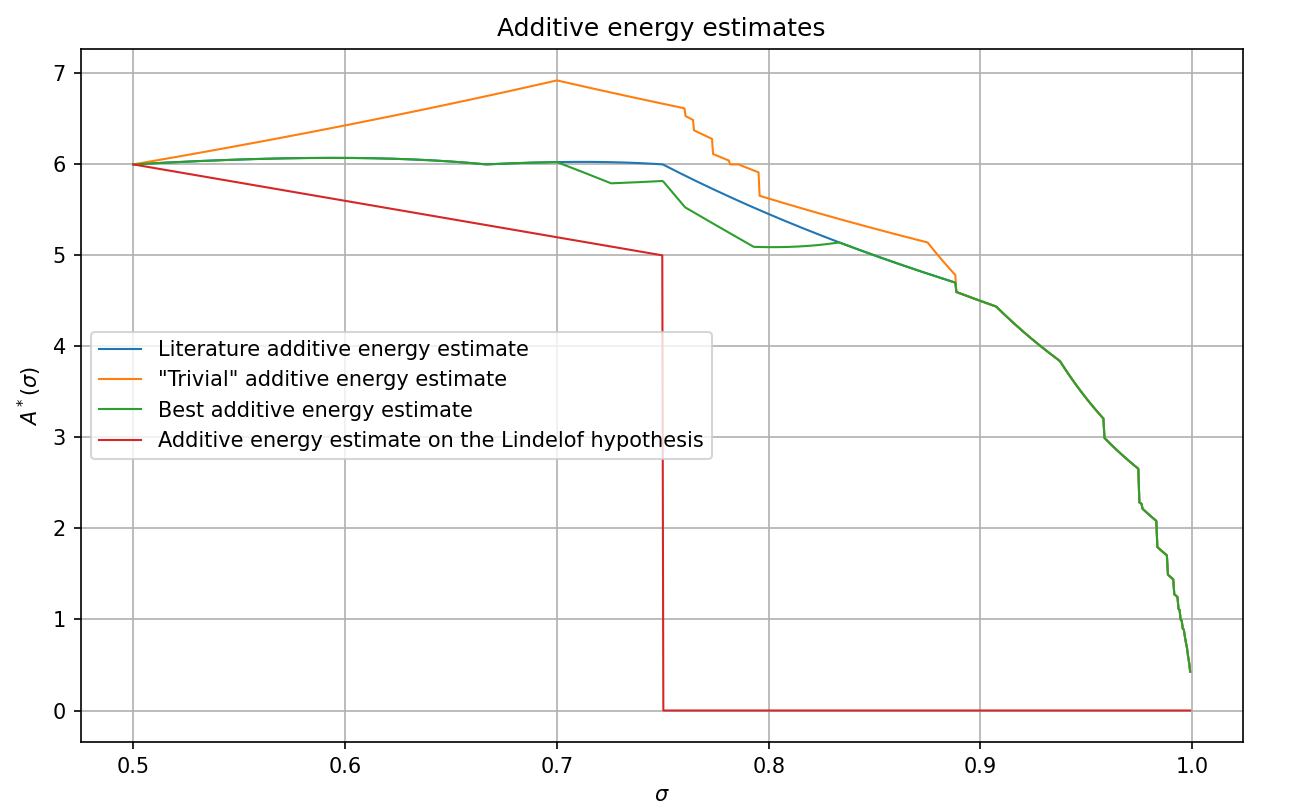
\includegraphics[width=0.5\linewidth]{chapter/zero_density_energy_estimate.png}
    \caption{Comparison of bounds on $\A^*(\sigma)$ under various assumptions.}
    \label{fig:zero_density_energy_estimate}
\end{figure}


